\section{Data handling and Training process}
\label{sec:datahandling}

\begin{figure}[H]
    \centering
    \begin{tikzpicture}[every node/.style={font=\tiny}]
        \tikzstyle{block} = [rectangle, rounded corners, draw=black, minimum width=2.5cm, minimum height=1.5cm, align=center, anchor=center]
    
        \newcommand{\emphasize}[1]{\scriptsize{\textbf{#1}}}
        \def\vsep{.6cm}
        \def\hsep{2cm}
    
        % linke Abfolge
        \node (image) at (0,0) [block] {\emphasize{Image} (RGB)};
        \node (Dataset)     [block, below=\vsep of image, align=center]     {\emphasize{Dataset}\\Data Augmentation\\out: [C, H, W]};
        \node (Dataloader)  [block, below=\vsep of Dataset, align=center]   {\emphasize{Dataloader}\\divides into batches\\out: [B, C, H, W]};
        \node (Model)       [block, below=\vsep of Dataloader, align=center]{\emphasize{Model}};
    
        % rechte Abfolge 
        \node (Video)       [block, right=\hsep of image, align=center]         {\emphasize{Video}};
        \node (Dataset2)    [block, below=\vsep of Video, align=center]         {\emphasize{Dataset}\\Data Augmentation\\out: [S, C, H, W]};
        \node (Dataload2)   [block, below=\vsep of Dataset2, align=center]      {\emphasize{Dataloader}\\divides into batches\\out: [B, S, C, H, W]};
        \node (TempModel)   [block, below=\vsep of Dataload2, align=center]     {\emphasize{Temporal Model}};
        \node (Sampler)     [block, right=.5*\hsep of Dataload2, align=center]  {\emphasize{Sampler}\\indexing for\\sequences};
    
        % Überschriften
        \node   [align=center, above=.2cm of image] {\emphasize{Single frame training Process}};
        \node   [align=center, above=.2cm of Video] {\emphasize{Temporal training Process}};
    
        \draw[-Stealth, thick] (image)       -- (Dataset);
        \draw[-Stealth, thick] (Dataset)     -- (Dataloader);
        \draw[-Stealth, thick] (Dataloader)  -- (Model);
    
        \draw[-Stealth, thick] (Video)            -- (Dataset2);
        \draw[-Stealth, thick] (Dataset2)         -- (Dataload2);
        \draw[-Stealth, thick] (Dataload2)        -- (TempModel);
        \draw[Stealth-Stealth, thick] (Dataload2) -- (Sampler);
        
    
    \end{tikzpicture}
    \caption{Comparison between data handling processes for single-frame training and the proposed temporal training.}
    \label{fig:dataHandlingProcess}
\end{figure}

The Dataset class reads images according to an index, performs online data augmentation, and outputs a tensor.
In the Dataset class, also the targets are formed from the augmented annotations.
First, Polylines are transformed into a mask, and then the data augmentation from \autoref{sec:dataaugmentation} is applied.
In the last step, this augmented mask is used to generate regression or classification targets.
For semantic segmentation, the mask can be utilized directly.
The Dataloader iterates through the dataset step by step and calls the dataset class using indices.
It can either move step by step or rely on a sampler to dictate the stepping pattern.
In temporal training, a sampler is essential for managing sequences, avoiding out-of-bound errors, and preventing scene intermixing.
A sliding window approach is implemented, shown in \autoref{fig:slidingWindow}.
A window of a predefined number of images serves as input for the model.
This number (usually 10) is smaller than the sequence length of 76.
Then, the data loader steps through the sequence.
At the end of a sequence, the sampler forces the Dataloader to jump to the next sequence instead of mixing them.
Furthermore, the Datalaoder creates batches and adds the dimension $B$ to the tensor.

\begin{figure}[H]
    \centering
    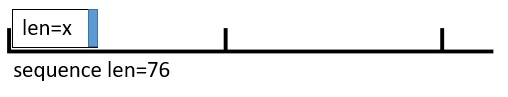
\includegraphics[width=0.5\linewidth]{PICs/usedDatasets/slidingWindow.jpg}
    \caption{Sampler is responsible for the sliding window approach in temporal training: bottom line represents the sequence with a length of 76 frames; the box is the window of frames used as the input for the model with x being the length of this window (with $x \leq 76$); the blue part of the sliding window represents the output frame because this temporal method deals with a sequence-to-one problematic.}
    \label{fig:slidingWindow}
\end{figure}

\noindent The training consists of a pre-defined number of epochs, which presents one training cycle.
In each epoch, the Dataloader feeds the model one batch.
Then, the model predicts, calculates the loss according to this prediction, and performs the back propagation to optimize the model.
In the same cycle, the validation is done, in which the Dataloader feeds the model samples of the validation set.
Here, only the prediction is done, and the loss is calculated.
Two additional steps are done in an epoch after training and validating.
On the one hand, the OneCycleLR scheduler \cite{pytorch_oneCycleLR_docu} is used to update the learning rate.
On the other hand, a model is saved as the best one as soon as it reaches a new minimum in the validation loss.
This way, the model with the lowest loss is obtained.
